\documentclass{article}

\usepackage{fullpage,enumitem,amsmath,graphicx}

\renewcommand\thesubsection{(\alph{subsection})}

\title{CS 224n Assignment \#2: word2vec}
\author{Heehoon Kim}
\date{}

\begin{document}

\maketitle

\section{Written: Understanding word2vec}

\begin{enumerate}[label=(\alph*)]
\item The one-hot vector $y$ is defined as the following formula.
\[
y_w=\begin{cases}
1,&\text{if }w=o\\
0,&\text{otherwise}
\end{cases}
\]
Thus,
\[
-\sum_{w\in Vocab}y_w\log(\hat{y}_w)=-y_o\log(\hat{y}_o)=-\log(\hat{y}_o).
\]
\item First, let's simplify $J$.
\[
\begin{split}
J_{naive-softmax}(v_c,o,U)&=-\log{P(O=o|C=c)}\\
&=-u_o^Tv_c+\log{\sum_{w\in Vocab}\exp u_w^Tv_c}
\end{split}
\]
The partial derivative is as follows:
\[
\begin{split}
\frac{\partial J_{naive-softmax}(v_c,o,U)}{\partial v_c}&=-u_o^T+\frac{1}{\sum_{w\in Vocab}\exp u_w^Tv_c}\sum_{w\in Vocab}(\exp u_w^Tv_c)u_w^T\\
&=-u_o^T+\sum_{w\in Vocab}P(O=o|C=c)u_w^T\\
&=-Uy+U\hat{y}\\
&=U(\hat{y}-y).
\end{split}
\]
\item When $w=o$,
\[
\begin{split}
\frac{\partial J_{naive-softmax}(v_c,o,U)}{\partial u_w}&=-v_c+\frac{1}{\sum_{w\in Vocab}\exp u_w^Tv_c}(\exp u_w^Tv_c)u_w^T\\
&=-v_c+P(O=o|C=c)v_c\\
&=v_c(\hat{y}_w-1).
\end{split}
\]
When $w\neq o$,
\[
\begin{split}
\frac{\partial J_{naive-softmax}(v_c,o,U)}{\partial u_w}&=P(O=o|C=c)v_c\\
&=v_c\hat{y}_w.
\end{split}
\]
\item Using $(f/g)'=(gf'-fg')/g^2$,
\[
\begin{split}
\frac{d\sigma}{dx}&=\frac{(1+e^{-x})1'-1(1+e^{-x})'}{(1+e^{-x})^2}\\
&=\frac{e^{-x}}{(1+e^{-x})^2}\\
&=\sigma(x)(1-\sigma(x)).
\end{split}
\]
\item The partial derivatives are as follows:
\[
\begin{split}
\frac{\partial J_{neg-sample}(v_c,o,U)}{\partial v_c}&=-\frac{1}{\sigma (u_o^Tv_c)}\sigma (u_o^Tv_c)(1-\sigma (u_o^Tv_c))u_o^T-\sum_{k=1}^{K}\frac{1}{\sigma (-u_k^Tv_c)}\sigma (-u_k^Tv_c)(1-\sigma (-u_k^Tv_c))(-u_k^T)\\
&=-(1-\sigma (u_o^Tv_c))u_o^T-\sum_{k=1}^{K}(1-\sigma (-u_k^Tv_c))(-u_k^T),\\
\frac{\partial J_{neg-sample}(v_c,o,U)}{\partial u_o}&=-(1-\sigma (u_o^Tv_c))v_c,\\
\frac{\partial J_{neg-sample}(v_c,o,U)}{\partial u_k}&=-(1-\sigma (-u_k^Tv_c))(-v_c).
\end{split}
\]
In case of $J_{naive-softmax}$, calculating the partial derivative with respect to $v_c$ requires matrix-vector multiplication of $O(|Vocab|\times (\text{word vector length})))$ time complexity.
On the other hand, calculating the derivative of $J_{neg-sample}$ only requires $K$ outside vectors. This results in $O(K\times (\text{word vector length})))$ time complexity, which is significantly fast if $K << |Vocab|$.
\item The partial derivatives are as follows:
\[
\begin{split}
\frac{\partial J_{skip-gram}(v_c,w_{t-m},...,w_{t+m},U)}{\partial U}&=\sum_{\substack{-m\leq j\leq m\\j\neq 0}}\frac{\partial J(v_c,w_{t+j},U)}{\partial U}\\
\frac{\partial J_{skip-gram}(v_c,w_{t-m},...,w_{t+m},U)}{\partial v_c}&=\sum_{\substack{-m\leq j\leq m\\j\neq 0}}\frac{\partial J(v_c,w_{t+j},U)}{\partial v_c}\\
\frac{\partial J_{skip-gram}(v_c,w_{t-m},...,w_{t+m},U)}{\partial v_w}&=0.
\end{split}
\]
\end{enumerate}

\section{Coding: Implementing word2vec}

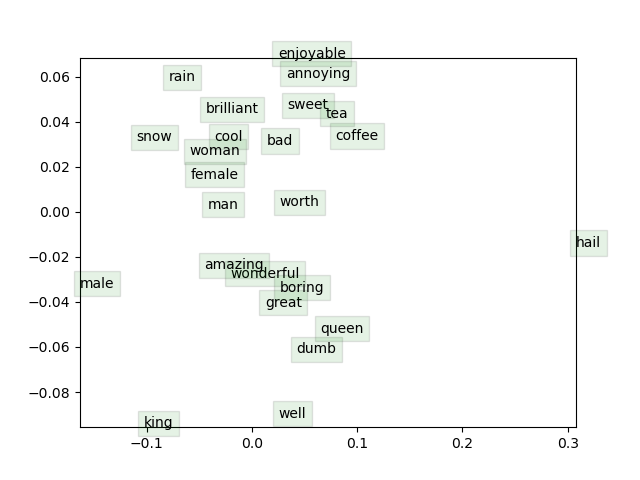
\includegraphics[width=\textwidth]{word_vectors}

\end{document}